%%%%%%%%%%%%%%%%%%%%%%%%%%%%%%%%%%%%%%%%%
% Twenty Seconds Resume/CV
% LaTeX Template
% Version 1.0 (14/7/16)
%
% This template has been downloaded from:
% http://www.LaTeXTemplates.com
%
% Original author:
% Carmine Spagnuolo (cspagnuolo@unisa.it) with major modifications by 
% Vel (vel@LaTeXTemplates.com) and Harsh Gadgil
%
% License:
% The MIT License (see included LICENSE file)
%
%%%%%%%%%%%%%%%%%%%%%%%%%%%%%%%%%%%%%%%%%

%----------------------------------------------------------------------------------------
%    PACKAGES AND OTHER DOCUMENT CONFIGURATIONS
%----------------------------------------------------------------------------------------

\documentclass[letterpaper]{twentysecondcv} % a4paper for A4

% Command for printing skill progress bars
\newcommand\skills{ 
~
    \smartdiagram[bubble diagram]{
        \textbf{Self-motivated}\\\textbf{Dev},
        \textbf{Relational/}\\\textbf{Document}\\\textbf{DB},
        %\textbf{~~~~OOP~~~~~},        
        \textbf{Latex/}\\\textbf{Markdown},
        \textbf{Web}\\\textbf{Stuff},
        \textbf{Machine}\\\textbf{Learning},
        \textbf{Deep}\\\textbf{Learning},
        \textbf{Hardware}\\\textbf{Programming},
        \textbf{Computer}\\\textbf{Vision}
    }
}

\interests{{Functional Programming/4.5},{ML DL/5},{Software Engineering/6},{Computer Vision/6}}

%----------------------------------------------------------------------------------------
%     PERSONAL INFORMATION
%----------------------------------------------------------------------------------------

% If you don't need one or more of the below, just remove the content leaving the command, e.g. \cvnumberphone{}



\cvname{{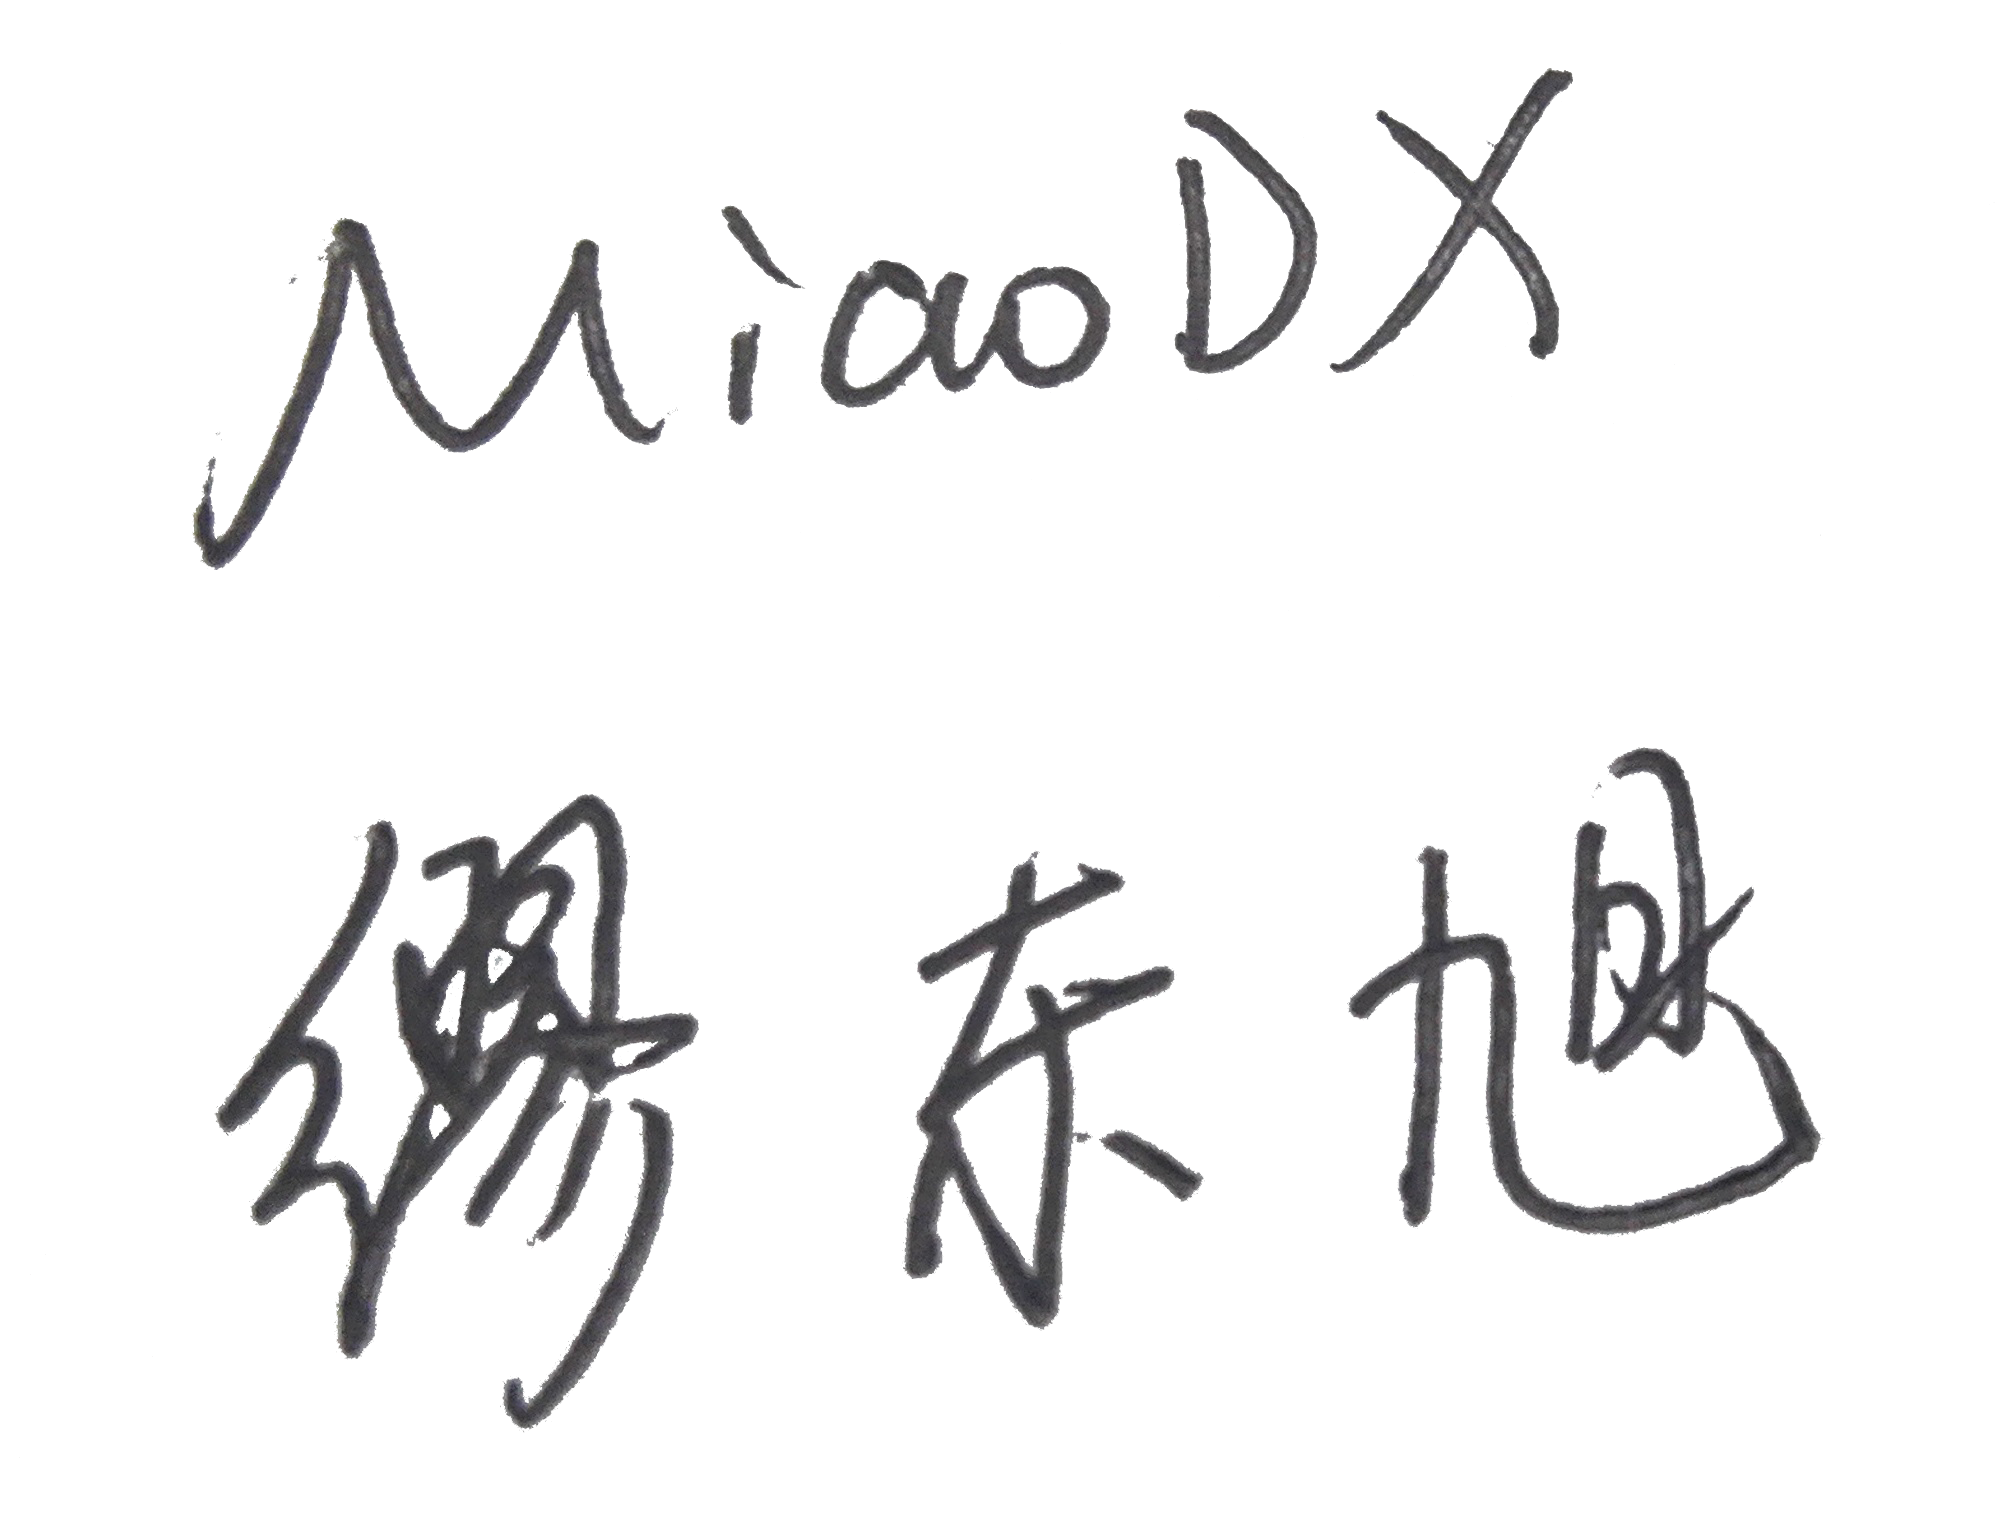
\includegraphics[scale=0.04]{img/miaodx_name.png}}} % Your name
\cvjobtitle{ Graduate Student, \\ Self-motivated Developer} % Job title/career

%\cvlinkedin{https://linkedin.com/in/miaodx}
\cvgithub{https://github.com/MiaoDX}
\cvnumberphone{+86 13502009660} % Phone number
\cvsite{https://miaodx.github.io/} % Personal website
\cvmail{miaodx@tju.edu.cn} % Email address

%----------------------------------------------------------------------------------------

\begin{document}

\makeprofile % Print the sidebar

%----------------------------------------------------------------------------------------
%     EDUCATION
%----------------------------------------------------------------------------------------
\section{Education}

\begin{twenty} % Environment for a list with descriptions
    \twentyitem
        %{Expected \\ Dec 2016}
        {2016 - Now}
        {MSe., Computer Software}
        {\href{http://tju.edu.cn/}{Tianjin University}}
        {Tianjin, China}
        {}
    \twentyitem
        {2012 - 2016}
        {BEng., Computer Software}
        {\href{http://www.xidian.edu.cn/}{Xidian University}}
        {Xi'an, Shaanxi, China}
        {}
    %\twentyitem{<dates>}{<title>}{<organization>}{<location>}{<description>}
\end{twenty}



\section{Scholarships \& Awards}

\begin{twenty}
    \twentyitem
        {2017-2018}
        {Second-class School Scholarship}
        {Tianjin University}
        {}
        {}
    \twentyitem
        {2016-2017}
        {First-class School Scholarship}
        {}
        {}
        {}
    \twentyitem
        {Oct 2016}
        {Postgraduate recommendation offer from Tianjin University}
        {}
        {}
        {}
    \twentyitem
        {2014-2015}
        {National Inspiration Scholarship}
        {Xidian University}
        {}
        {}
    \twentyitem
        {2014CUMCM}
        {Second-class prize in Shaanxi Division}
        {}
        {}
        {}
    \twentyitem
        {2013-2014}  
        {Second-class School Scholarship}
        {}
        {}
        {}
    \twentyitem        
        {2012-2013}
        {First-class School Scholarship}
        {}
        {}
        {}        
\end{twenty}

\section{Papers}

\begin{twenty}
    \twentyitem
        {Jan 2018}
        {Paper Accpeted by ICASSP 2018}
        {}
        {}
        {ACTIVE CAMERA RELOCALIZATION WITH RGBD CAMERA
FROM A SINGLE 2D IMAGE (Camera ready, First Author)}
\end{twenty}

\section{Projects}
\begin{twenty}

    \twentyitem
        {}
        {Recent projects, more can be found on github}
        {\href{https://github.com/MiaoDX/}{github.com/MiaoDX}}
        {}
          {}
          
    \twentyitem
    {Jan 2018 - \\ Present}
    {ICRA 2018 DJI ROBOMASTER AI CHALLENGE}
    {}
    {}
    {Preparing for ICRA 2018 DJI ROBOMASTER AI CHALLENGE with other five teammates from TJU.}              
          
          
    \twentyitem
        {Virtual Env \\ DL}
        {Unrealcv with DL (Faster-RCNN)}
        {\href{https://github.com/MiaoDX/unrealcv_examples/}{Unrealcv with DL}}
        {}
        {Integrate one tensorflow faster rcnn implement (\href{https://github.com/smallcorgi/Faster-RCNN\_TF}{smallcorgi/Faster-RCNN\_TF}) with virtual environment library \href{https://github.com/unrealcv/unrealcv}{unrealcv}. Exploring the potential benefits of synthetic data on improving exisiting DL implements.}          
                 
    \twentyitem
        {Python \\ RL}
        {PacMan capture the flag with Reinforcement Learning}
        {\href{https://github.com/MiaoDX/hand_in_homework/tree/master/Advanced\_AI/}{PacMan with RL}}
        {}
        {Some reinforcement projects on pacman capture the flag game, with fundamental concepts and a contest hold in class.}


    \twentyitem
        {OpenCV}
        {Notes on OpenCV}
        {\href{https://github.com/MiaoDX/opencv\_projects/}{opencv\_notes}}
        {}
        {Notes, example codes and some tricks for working with OpenCV.}

\end{twenty}



\begin{twenty}

    \twentyitem
        {Python \\ ML}
        {UCI Adult database processing with scikit-learn}
        {\href{https://github.com/MiaoDX/scikit\_learning/}{scikit\_learning}}
        {}
        {Use scikit-learn to predict whether income exceeds \$50K/yr based on census data, got the best result in class(85\%-86\% precision on test set with scikit-learn lib only).}


        
    \twentyitem
        {Java \\ BP}
        {A sample back propagation implementation using java}
        {\href{https://github.com/MiaoDX/bp_java}{bp\_java}}
        {}                
        {I think it really necessary to implement a simple ANN from scratch before diving into those amazing open source ML(\/DL) libraries. In this way, we will have a better understanding of ANN and will not treat those toolkits as black-boxes and just hope we will get nice result after an uncertain time.}

    \twentyitem
        {Node.js \\ mongodb}
        {Attendance management system}
        {\href{https://github.com/SEAPC2016/attendance}{attendance system}}
        {}
        {In a team of four, made an RESTful attendace webset system with Node.js, mongodb and Jade for a (faked) company. Stuffs can ask for leave via our system and wait for the managers's approval, statistical information can also be generated from our system.}

        
%    \twentyitem
%        {Baidu Map API  \\ D3.js}
%        {Display churches in Tianjin}
%        {\href{https://github.com/MiaoDX/baidu\_map\_church}{baidu\_map\_church}}    
%        {}
%        {Course project of Visual Analysis class, since I really love the architecture of old churches, so I use Baidu Map API to get all churches' locations in Tianjin and display them with D3.js.}    


\end{twenty}


\section{Experience}

\begin{twenty}

\twentyitem
    {Feb 2017 - \\ July 2017}
    {Graduate Teaching Assistant}
    {\href{http://tju.edu.cn/}{Tianjin University}}
    {}
    {TA for Programming Design Practice I, full English course for freshmen.}    

\twentyitem
    {Feb 2017 - \\ May 2017}
    {Teaching Python101}
    {\href{https://github.com/MiaoDX/python101}{MiaoDX/python101}}
    {}
    {Teaching python for several master students major in finance for their preparing for overseas study.}    

\twentyitem
    {Summer vacation \\ 2013}
    {Valunteer Teacher}
    {\href{http://blog.sina.com.cn/xiaanedu}{Dripping Action}}
    {}
    {I volunteered to teach in a primary school in TongChuan, Shannxi province for more than half a month(18 days) with my teammates, that volunteer work was organized by “Dripping Action”(one project of Mutualistic Symbiosis Community of Youths \& Environment, Shaanxi).
    }


\twentyitem
    {Sep 2012 - \\ Sep 2013}
    {Club activity}
    {\href{http://www.xidian.edu.cn/}{Xidian University}}
    {}
    {Member of Young Volunteer team and Work-study centre clubs in
School.}    


    
    
\end{twenty}

\section{Personal}

\begin{twenty} % Environment for a list with descriptions
    
\twentyitem
    {}
    {}
    {}
    {}
    {        
        {\begin{itemize}
            \item Passed CET-6 (460), English as working language
            \item Reading, Boxing, Running, Cycling
        \end{itemize}
         }
    }    
        
    %\twentyitem{<dates>}{<title>}{<location>}{<description>}
\end{twenty}

\end{document} 
